% !TeX root = main.tex

\hypertarget{linearization}{%
\section{Linearization}\label{linearization}}

Let \(f\) be a function differentiable at \(x=a\). Then for a number
\(x\) near \(a\), the value of the function \(f(x)\) can be approximated
using the tangent line \(y=f'(a)(x-a)+f(a)\).

That is \[f(x)\approx f'(a)(x-a)+f(a)\] We call the function
\(L(x):=f'(a)(x-a)+f(a)\) the \textbf{\emph{linearization}} or
\textbf{\emph{linear approximation}} of \(f\) at \(a\).

\begin{example}

Find the linearization of \(f(x)=\sqrt{x}\) at \(x=1\) and estimate
\(f(1.01)\). \url{https://www.desmos.com/calculator/urjragsxae}

\end{example}
\vspace*{6\baselineskip}

\begin{example}

Find the linearization of \(f(x)=\cos x\) at \(x=60^\circ\) and estimate
\(\cos(61^\circ)\).

\end{example}
\vspace*{6\baselineskip}

\begin{example}

Estimate the value of \(\sqrt[3]{0.98}\) using local linear
approximation for the function \(f(x)=\sqrt[3]{1+x}\).

\end{example}
\vspace*{6\baselineskip}

\hypertarget{differentials}{%
\subsection{Differentials}\label{differentials}}

Sometimes, we only need to know the relative change. The linear
approximation provides an estimate of the relative change in the
dependent variable \(y\) using the relative change of the independent
variable \(x\). Suppose that \(y=f(x)\). We denote by \(\mathrm{d}x\)
the change in \(x\) which can be assigned with any value, and define
\[\mathrm{d}y=f'(x)\mathrm{d}x.\] Then \(\mathrm{d}y\) can be viewed as
a function of \(\mathrm{d}x\). We call \(\mathrm{d}x\) and
\(\mathrm{d}y\) \textbf{\emph{differentials}}.

Given that \(f\) is differentiable at \(a\) and \(\mathrm{d}x\) is
small, the value \(f(a+\mathrm{d}x)\) is approximately

\[
f(a+\mathrm{d}x)\approx L(a+\mathrm{d}x)=f(a)+f'(a)(a+\mathrm{d}x - a).
\]

Then the actual change \(\Delta y=f(a+\mathrm{d}x)-f(a)\) is
approximately

\[
\Delta y=f(a+\mathrm{d}x) - f(a)\approx L(a+\mathrm{d}x) - f(a)=f'(a)\mathrm{d}x=dy.
\]

\begin{fullwidth}
  \centering
  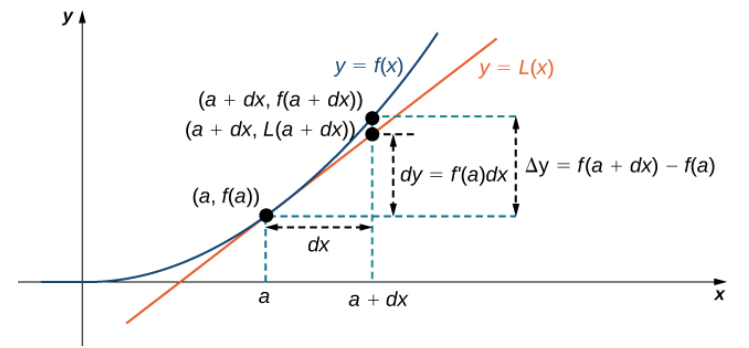
\includegraphics[scale=0.5]{img/image-20201017200202969.png}
\end{fullwidth}

\begin{example}

Find the differential \(\mathrm{d}y\) for the function \(y=x^3-\frac1x\)
and evaluate for \(x=1\) and \(\mathrm{d}x=0.01\).

\end{example}
\vspace*{6\baselineskip}

\begin{example}

Let \(y=tan(5x+2)\). Using the differential to estimate \(\Delta y\)
when \(x=1\) and \(\mathrm{d}x=0.4\).

\end{example}
\vspace*{6\baselineskip}

\hypertarget{applications-and-measurement-errors}{%
\subsection{Applications and Measurement
Errors}\label{applications-and-measurement-errors}}

In application, due errors in measurement, if a quantity is calculated
based on a measurement, it is likely subject to an error too. This type
of error is known as a \textbf{propagated error}. Suppose the quantity
is determined by a function \(f\) of the measurement \(x\). If the
measurement has an error \(\mathrm{d}x\), then the propagated error
\(f(a+\mathrm{d}x)-f(a)\) is approximately \[
\Delta y=f(a+\mathrm{d}x)-f(a)\approx f'(a)\mathrm{d}x=dy.
\]

\begin{remark}

\begin{remark}

When \(f'(x)\) is continuous, if we don't know \(a\), by continuity, we
may the measured value \(a+\mathrm{d}x,\) to estimate the propagated
error

\[
\Delta y\approx dy\approx f'(a+\mathrm{d}x)\mathrm{d}x.
\]

\end{remark}

\end{remark}

\begin{example}

Suppose the side length of a cube is measured to be 2 cm with an
accuracy of 0.1 cm.

\begin{enumerate}
\item
  Use differentials to estimate the error in the computed volume of the
  cube.
\item
  Compute the volume of the cube if the side length is (a) 1.9 cm and
  (b) 2.1 cm to compare the estimated error with the actual potential
  error.
\end{enumerate}

Given an absolute error \(\Delta q\) for a particular quantity, we
define the relative error as \(\frac{\Delta q}{q}\), where \(q\) is the
actual value of the quantity.

\end{example}

\begin{example}

An astronaut using a camera measures the radius of Earth as 4000 mi with
an error of \(\pm 80\) mi. Let's use differentials to estimate the relative
and percentage error of using this radius measurement to calculate the
volume of Earth, assuming the planet is a perfect sphere.

\end{example}
\vspace*{6\baselineskip}

\subsection{Practice}

\begin{exercise}

Find the linearization of \(f(x)=\sqrt[3]{x}\) at \(x=8\) and estimate
\(f(8.03)\).

\end{exercise}
\vspace*{6\baselineskip}

\begin{exercise}

Find the linearization of \(f(x)=\sec x\) at \(x= 45^\circ\) and
estimate \(f(44^\circ)\).

\end{exercise}
\vspace*{6\baselineskip}

\begin{exercise}

Find \(\mathrm{d}y\) for \(y=\sqrt[n]{x+1}\) and evaluate when \(x=0\)
and \(\mathrm{d}x=0. 01\), where \(n\) is a positive integer.

\end{exercise}
\vspace*{6\baselineskip}

\begin{exercise}

Find \(\mathrm{d}y\) for \(y=\sin\left(\dfrac{\pi x+\pi}{2}\right)\) and
evaluate it when \(x=0\) and \(\mathrm{d}x =0.01)\).

\end{exercise}
\vspace*{6\baselineskip}

\begin{exercise}

Estimate the value of \(\displaystyle \frac{6}{\sqrt{1-x}}\) at
\(x=0.01\) using linear approximation.

\end{exercise}
\vspace*{6\baselineskip}

\begin{exercise}

The circumference of a sphere was measured to be 73 cm with a possible
error of 0.5 cm.

\begin{enumerate}
\item
  Use linear approximation to estimate the maximum error in the
  calculated surface area.
\item
  Estimate the relative error in the calculated surface area.
\end{enumerate}

\end{exercise}

\begin{exercise}

Let \(y=\sin(5x)\).

\begin{enumerate}
\item
  Estimate \(\sin(0.5)\) using linear approximation.
\item
  Find the percentage error
\end{enumerate}

\end{exercise}

\begin{exercise}

Use linear approximation to estimate the amount of paint in cubic
centimeters needed to apply a coat of paint 0.05 cm thick to a
hemispherical dome with a diameter of 40 meters.

\end{exercise}

